\documentclass[aps]{revtex4}
\usepackage{natbib}
\usepackage{graphics} % use the graphics package for simple commands
\usepackage{graphicx}
\usepackage{amsmath}
\usepackage{amssymb} % The amssymb package provides various useful mathematical symbols
\usepackage{fdsymbol}
\usepackage{wrapfig}

\usepackage{pstricks}
%\usepackage{cite}
%\usepackage[symbol]{footmisc}
%\renewcommand{\thefootnote}{\fnsymbol{footnote}}

\newcommand{\ket}[1]{\ensuremath{\left| #1 \right\rangle}}
\newcommand{\bra}[1]{\ensuremath{\left\langle #1 \right|}}
\newcommand{\braket}[2]{\ensuremath{\left\langle #1 \right|\left. #2 \right\rangle}}
\newcommand{\expect}[1]{\ensuremath{\left\langle #1 \right\rangle}}
\newcommand{\eV}{\mbox{eV}}
\newcommand{\icm}{\ensuremath{\mbox{cm}^{-1}}}
\newcommand{\cm}{\mbox{cm}}
\newcommand{\EE}[1]{\ensuremath{\times 10^{ #1 }}}
\newcommand{\ee}[1]{\ensuremath{\times 10^{ #1 }}}
\newcommand{\norm}[1]{\ensuremath{\left| #1 \right|}}
\newcommand{\abs}[1]{\ensuremath{\left| #1 \right|}}
\newcommand{\HH}{\mathcal{H}}
\newcommand{\laplace}[1]{\ensuremath{\mathcal{L}\left\{ #1 \right\}}}
\newcommand{\fourier}[1]{\ensuremath{\mathcal{F}\left\{ #1 \right\}}}
\newcommand{\invlaplace}[1]{\ensuremath{\mathcal{L}^{-1}\left\{ #1 \right\}}}
\newcommand{\invfourier}[1]{\ensuremath{\mathcal{F}^{-1}\left\{ #1 \right\}}}
\newcommand{\myexp}[1]{\ensuremath{ \exp\left( #1 \right) }}
\newcommand{\eps}{\varepsilon}
\newcommand{\myerf}[1]{\ensuremath{{\mathrm{erf}\left( #1 \right)}}}
\newcommand{\heaviside}[1]{\ensuremath{ \mathrm{\Theta}\left( #1 \right)}}
\newcommand{\etal}{,~\textit{et~al.,~}}


\usepackage{times}

\graphicspath{{./figs/}} % Change Graphics Path for figs and institution logo.
%\setlength{\parindent}{.05\linewidth}

\begin{document}

\title{Enabling Long Wavelength Streaking for Attosecond Science\\FWP 100498}

\author{Audrey Corbeil-Therrien, Debadri Das, Matt Feldman, Averell Gatton, Kunle Olukotun, Amedeo Perazzo, Omar Quijano, Peter Walter, and Ryan N. Coffee}
%\author{Audrey Corbeil-Therrien\footnotemark, Debadri Das\footnotemark, Matt Feldman\footnotemark, \setcounter{footnote}{0} Averell Gatton\footnotemark, Kunle Olukotun\setcounter{footnote}{2}\footnotemark, Amedeo Perazzo\setcounter{footnote}{0}\footnotemark, Omar Quijano\setcounter{footnote}{0}\footnotemark, Peter Walter\setcounter{footnote}{0}\footnotemark, and Ryan N. Coffee\setcounter{footnote}{0}\footnotemark \setcounter{footnote}{3}\footnotemark\\
%\setcounter{footnote}{0}\footnotemark LCLS \hspace{24pt} \footnotemark Stanford Applied Physics \hspace{24pt} \footnotemark Stanford EE/CS \hspace{24pt}\footnotemark The PULSE Institute, SLAC National Accelerator Lab, 2575 Sand Hill Road, Mail Stop 20, Menlo Park, California 94025}

\newlength{\figwidth}
\setlength{\figwidth}{.9\linewidth}

\maketitle

%---- Body ----%
\subsection*{Project Identification}
We present an update of the project entitled ``Enabling Long Wavelength Streaking for Attosecond Science.''
This effort is a co-design approach that targets an optimized next generation of angular array of electron Time-of-Flight (aa-ToF) detectors, often refered to as a ``Cookiebox.''

\subsection*{Accompolishments}
\begin{itemize}
\item Initial measurement of MCP raw waveforms for use in signal simulations for analysis model development.
\item Preliminary design of ToF complete and included in signal simulations.
\item Purchase of Flange Assembly for mounting MCP assembly in euv lab chamber for testing.
\item Two options identified for retardation, the multi-blade stack and tailored Silicon Carbide.
\item Initial demonstration of machine learning for x-ray pulse reconstruction, now exploring leaner networks for sake of FPGA compatibility.
\item Purchase of upgraded digitizer modules based on pulse reconstruction needs and simulations.
\item Working Docker containers for both full simulation as well as ML training and inferencing of x-ray pulse waveform based on streaking simulation.
\end{itemize}

\begin{wrapfigure}[15]{l}{.4\linewidth}
\centerline{\includegraphics[clip,width=\linewidth]{FlangeAssembly2.eps}}
\caption{\label{fig::taran}
The Hamamatsu detectors are mounted to 6 inch vacuum flanges as shown.
}
\end{wrapfigure}

%In the email I just sent, the waveform images for 1600 and 400 correspond to average central number of hits. The 400 has been scaled to have the same input magnitude of the waveforms as the 1600. This shows that if our probability distribution from the kernel density estimate is scaled appropriately, then we can expect similar results from sampling 1600 vs 400. Keep in mind this has not been tested with random background electrons, which may degrade the signal by quite a bit.. 
%Also, what I am seeing here is that we are going to have to have a big model to reconstruct at .25eV. 
%In short:
%We win at reducing the count rate.
%We loose at constructing SASE substructure (currently) -- research ongoing into more better ML.
%-Ave


%For the characterization of the MCP response at PULSE/design for mounting the MCPs on the back of the TOF tubes:
%- Flange design complete.
%- All parts required to be machined for prototype (which will also be used for the test at PULSE) have been made.
%- All other part orders for prototype placed, all parts arrived except for feedthroughs, spacer flange and custom multiport flange.
%- The bottleneck is the multiport flange, which is scheduled to be completed to ship by 4/23. Once it arrives we can build and install straight away.

%Machine learning and simulation:
%-- in the process of testing model architectures for what gives the best fit. Attempting to create the best possible model regardless of whether it will fit on a GPU.
%        -- testing models based on the number of hits, energy resolution, stability of inference against random noise etc. Hopefully this tells us if we can live with less counts per shot.
%	- Simion: simulating what the resolution is for no mesh spectrometers
%	- Mesh bending: this week will order lenses and mirror blanks and test mesh.
%	- SiC will also order these parts this week. 
%	- Auto-Cad: asked Mike about getting set up with Autocad to do some preliminary drawings.
%
%Initial working Docker container for spatial-lang and vivado with initial development of pipelined convolution kernels. 





\textbf{Publications, conference papers, patents: }
Although we have not had any publications or conference proceedings to date, we note that this effort has been featured in a co-design workshop hosted by SLAC, was featured in the SLAC Faculty retreat as a presentation on EdgeML, and also featured in the recent XFEL Sase 4/5 workshop.


\subsection*{Collaborations }
Corbeil-Therrein has submitted an FPGA-chaining LDRD proposal together with members of TID-AIR related to a general paradigm of FPGA-based machine learning inference that spans both on sensor FPGAs and larger EdgeML compute node FPGAs.
We are actively working with the L2SI PCDS effort in co-developing the digitizers via bi-weekly meetings; our ``CookieBox'' has become a ``poster child'' for data reduction and low-latency data sort and veto triggers.
TMO lead Peter Walter is co-investigator on this project and has begun project ``MRCOFFEE'' which will use the output of this FWP to specify the requirements for a full 16-fold angular array detector for user availability in IP1 of Hutch 1.1.
Stanford CS/EE Matt Feldman developing an FPGA compilation environment based on spatial-lang as a potential alternative to the SLAC RCE Platform being developed within TID-AIR for general purpose upstream  FPGA logic.
The LCLS Laser Team is targeting a laser module for IP1 in TMO that is aimed at long wavelength optical lasers for infrared optical streaking style experiments.

A key collaborator is one of the PI's former post-doctoral fellows, Markus Ilchen.  
Ilchen is currently a research scientist at the European XFEL where he and another long time colleague Gregor Hartmann are making early test of signal degredation at the high repetition rates xFEL.
These test are directly informing our decisions not only on the detector hardware but also on the analysis logic that determines the FPGA resources needed in the digitizers.


\subsection*{Impact}
Immediately, the successful outcome of this FWP would provide a new way to do high resolution attosecond time-resolved electron spectroscopy with angle resolution as an alternative to the low signal per event mode of reaction microscopes.  
It will open angular streaking as a way to access sub-femtosecond scale physics.

The CookieBox project is also our poster child for EdgeML co-design given it's potential to produce many hundreds of GB/s.
It is our most immediate ``firehose'' data source whose low-latency inference output could be used to route, veto, or sort data in downstream detectors.
It gives us early insight into allowing user-defined ML models for low-latency automation at high data throughput user facilities.  


\subsection*{Changes and challenges}
We are coordinating with the L2SI project regarding engineering and design support in order to maintain a September target for the final design of the ToF modules and chamber.
We expect to place orders for fabrication in September or October.

March data from EuroXFEL, courtesy of collaborators Gregor Hartmann and Markus Ilchen, has shown us that MCPs will not survive a 50 counts/shot rate at cw 1MHz.
Since we are targeting 1MHz cw operation, we have been forced to reduce the number of detected electrons per shot and instead rely more heavily on Kernel Density Estimation to account for the undersampling of the photoelectron momentum distribution.
Furthermore, we have paused the order of the planned MCP assemblies and will test an identical MCP assembly but with smaller pore diameter in the hopes that we will find a faster response time and smaller gain.
Ironically, the gain in the MCPs is our enemy; we much prefer a better time--and therefore energy--resolution and lower charge electron cascades per count.
Furthermore, excess noise from retardation grids is pushing us to simulate a gridless design.

The accelerated schedule is motivating the early purchase of hardware and fabrication of the chamber in late FY19 or at latest very early FY20.
Advancing the schedule will accommodate the long lead time for mu-metal chamber fabrication while preserving the ability to use intermittent access to Hutch 1.1 during Run 18.
Run 18 operation begins in April 2020 and so targeting the end of Run 18 will allow that this detector could be tested against multi-pulse FEL modes even at 120 Hz LCLS soft x-ray operation before the FY21 start of LCLS-II.

The digitizers are now in a second upgrade phase as a result of our preliminary results.
Our detector development inspired the L2SI project to upgrade the base digitizer to the Abaco FMC134 + PC821 carrier which uses a Xilinx Kintex Ultrascale KU085 FPGA.  
In return they have purchased an early testing example of this KU085 model.
In developing the pre-analysis logic based on the measured impulse response, signal simulations, and hit rate limitations learned from EuroXFEL tests, we plan to use two waveforms that measure waveforms from 90 degree separated ToF modules.
This allows a more tightly constrained Kernel Density Estimation when inverting the under-sampled the photoelectron momentum probability distribution.
We plan to push that logic to the FPGA that resides on the digitizer carrier card.
Since the base KU085 model has very little excess logic and DSP blocks remaining after the digitization logic, we will upgrade to the Ultrascale KU115 FPGA.
The extra 50\% logic, memory, and DSP resources will effectively double the computational resources for on-digitizer preprocessing.


\subsection*{Budgetary information}
\paragraph*{Labor \& Indirect}
Audrey Corbeil-Therrein and Averell Gatton are each support at the 0.5 FTE level for a total of 1FTE post-doc support for the duration of the project.
We also include 240 hours of shop labor which is expected to be used predominantly in FY20. 
The total labor cost is therefore \$242.2k.
The indirect cost for the project is \$188.1k.

\paragraph*{Materials \& Supplies}
The total expected budget for equipment, with updated quotes and updated parts where needed, is expected at the \$215.8k level.
We note that this is \$32.8k above the original estimate of \$183k for materials and supplies.
This is \$32.8k above the originally proposed estimate but only \$6.8k above the received funds as of April 2019.
At this level, we expect to slightly adjust the labor levels for FY20 to cover this amount.

The main vacuum chamber is in design phase but is expected to be on the scale of \$40k and scheduled for order to be placed late August or early September.
%Digitizer + Carrier board = 25k x 4,  22.5k + 1.6Kupgrade form KU085->KU115 call it 25 K for the carrier card and FPGA.
%100k (75k) digitizers
We have ordered 3 units of the Abaco Inc. model PC821 carrier card with the Xilinx XCKU115 FPGA with the FMC134 6.4~GSps, 2 channel digitizer at \$75K total.
We note that the 4th needed unit for a set of 8 detectors has already been purchased, although with the lower grade Xilinx XCKU085 FPGA option, by the L2SI budget and will be used for comparative testing.
We have initiated the purchase of the smaller pore diameter model of the Hamamatsu MCPs to test for differences in the response at high count rate.
These first two are expected at a cost of \$14.2k total, followed by an additional 6 units for a total project cost of \$56.8k
The 6 inch vacuum flange and feedthrough assembly as shown in Fig.~\ref{fig::taran} is straightforward and so purchase two units at \$5.5k per flange have been made and the following 6 units will be ordered after benchmark tests scheduled for mid to late May; we expect a total cost of \$44k for all feedthough flanges.

%23K labor so far:
%122+120 labor in budget

%New budget 240.8k total: (other direct cost)
%57.2 higher cost than original.
%640k - 614k orig = 26k

%Original Budget 183k total: (other direct cost)
%40K chamber FY19
%42.6K MCP electronics x6
%66k digitizers
%6K computer
%9K Xilinx KCU1500 FPGA
%6K FPGA streaming analysis
%14K M&S vacuum



\paragraph*{Leveraged contributions}
This project benefits heavily from the 
Ryan Coffee is supported at the 30\% level via LCLS Soft X-ray Research departmental support and 20\% through the MLDRP-LDRD effort through the end of FY19. 
Peter Walter is supported via LCLS Soft X-ray Research departmental support and the L2SI project.  
James Cryan is support through via LCLS Soft X-ray Research departmental support and also has committed to his High Harmonic euv source for testing of the MCP electronics in the PULSE lab.
Averell Gatton is funded 50\% via LCLS Soft X-ray Research departmental support for post-doctoral researchers.
Audrey Corbeil-Therrein is 50\% funded via a Canadian Post-Doctoral Fellowship.
Taran Driver is supported at the 50\% level via LCLS Soft X-ray Research departmental support for post-doctoral researchers.
Debadri Das is supported at the 50\% by LCLS Photon Control and Diagnostic Systems student support.

The ``Machine Learning for the Data Reduction Pipeline'' (MLDRP) project is a Lab Directed Research and Development (LDRD) project that is contributing not only labor support for Coffee and Quijano, but also an EdgeML computing node.
This compute node is used for both the simulation and ML training discussed above.
It has a large PCIe bus that will house the digitizers and FPGA processing for the early euv testing in the PULSE lab.
Also via the MLDRP project, Matt Feldman effort is leveraged as a Stanford Graduate Fellowship via collaboration with Kunle Olukotun in Stanford Computer Science and Electrical Engineering.
Omar Quijano is supported at the 20\% level through Photon Control and Diagnostic Systems department.

The LCLS Accelerator R\&D budget contributed the initial Hamamatsu detector assembly that was used for measuring the MCP response function that servs as our basis for simulation and design. 

In January 2019, the L2SI budget ordered one of the base digitizer plus carrier card to accommodate the early MCP testing in mid May so as to coincide with the scheduled delivery of the initial two flanges and MCP assemblies.

\paragraph*{Initial funding}
Initial funding began at the end of FY18 with \$290k.  Fiscal year 2019 funding has now fully arrived at the level of \$350k for a total of \$640k. 
The motivation for advancing the funding into FY19 is to accommodate the long lead time associated with mu-metal chamber fabrication and the intermittent access to Hutch 1.1 during Run 18 operation which begins in April 2020.
We therefore expect to finalize the integrated ToF modules and chamber design and be ready for order by September of 2019.  
This schedule allows for a 6 month fabrication schedule and then a 6 month installation schedule to be ready by close of FY2020.
This schedule is aligned with the potential for an October 2020 high repetition rate LCLS-II availability in hutch 1.1 for detector testing, demonstration, and resolution benchmarking.

\subsection*{Funds spent to date}
0.5 FTE for first half of FY19 support of Gatton and Corbeil-Therrien.
\$11k for initial flanges for testing, to arrive in mid-May.
\$75k for digitizers ordered to arrive by FY19-end.
\$14.2k for 2 units of small pore MCP assemblies for testing to arrive by late summer 2019. 

\bibliographystyle{unsrt}
\bibliography{$BIBFILES/Coffee,$BIBFILES/computing}

\section*{Acknowledgements}
%It is under B&R (Budget & Reporting) code KC0406020.
This work is supported by the U.S. Department of Energy, Office of Science, Office of Basic Energy Sciences under Contract No. DE-AC02-76SF00515.
The CookieBox effort is supported under the Accelerator and Detector Research program of the U.S. Department of Energy, Office of Science.
The EdgeML effort is supported by the Department of Energy, Laboratory Directed Research and Development program at SLAC National Accelerator Laboratory.
Feldman is supported by the Stanford Graduate Fellowship in Science and Engineering.
Corbeil-Therrien is partially supported through a Banting Postdoctoral Fellowship from the Government of Canada.


\end{document}


\pagebreak


\section{Data Pipeline}

Motivating co-design, we look for a pipelined algorithm that fits into the spare digitizer FPGA logic that also relaxes our need to record multiple electron hits in so-called ``current'' mode.

\begin{wrapfigure}[40]{r}{.5\linewidth}
\centerline{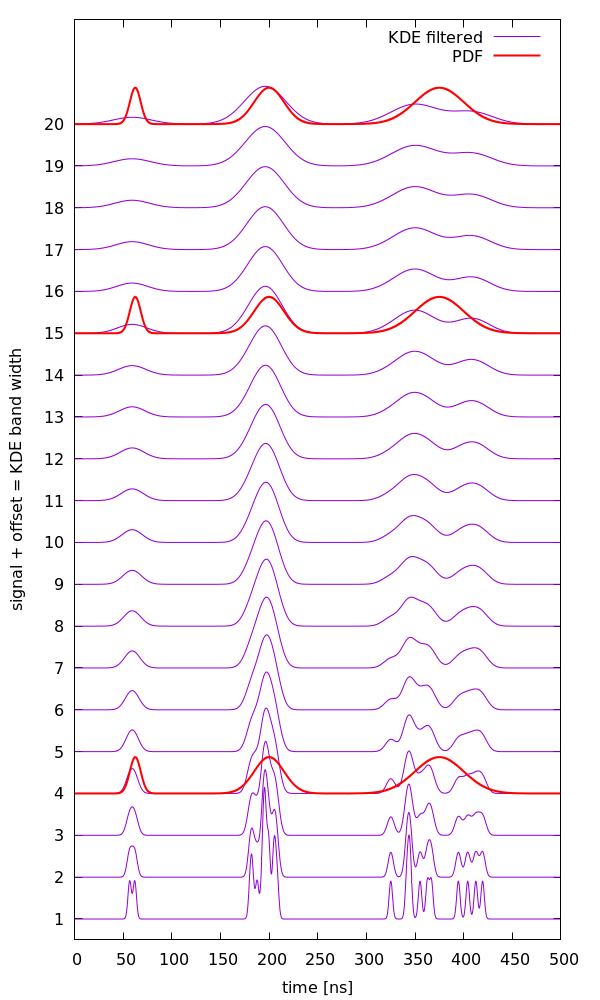
\includegraphics[clip,width=\linewidth]{dynamic.kernel.motivation.eps}}
\caption{\label{fig::kde}
Here we show Kernel Desity Estimation (KDE) in blue by varying the bandwidth the kernel that is applied to the electron hits associated with the under-sampled probability distribution functions (PDFs), shown as red, as described in the text.
}
\end{wrapfigure}

\begin{figure}
\centerline{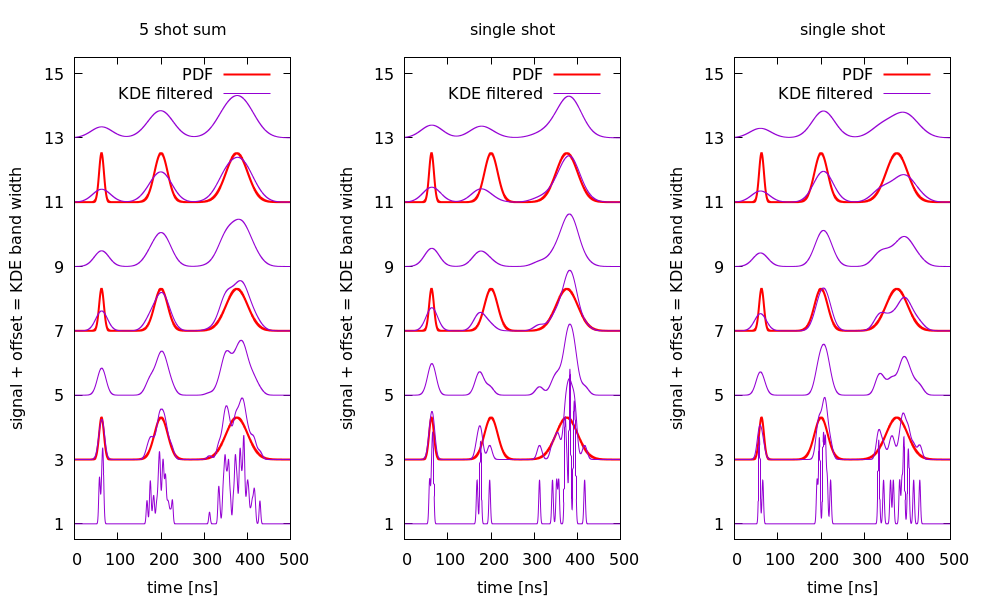
\includegraphics[clip,width=\figwidth]{dynamic.kernel.motivation.multi.eps}}
\caption{\label{fig::multi_single_kde}
Here we compare the case of multiple (5) shots averaged together (left) with single shot cases with undersampled probability distrbutions (center and right).
}
\end{figure}

\section{Conclusion}
\section*{The CookieBox}

The CookieBox project is a recently funded (FY19-FY20) project under the DOE Accelerator and Detectors Research program.
This project, formally titled ``Enabling long wavelength streaking for attosecond x-ray science'' aims to produce a prototype detector system that demonstrates an optimal balance between electron time-of-flight (ToF) spectral resolution and collection efficiency.
The detector is optimized for attosecond angular streaking \cite{Nick2018,Siqi2018} for x-ray pulse characterization at full LCLS-II repetition rates.
The output of this project will feed the design specifications for the ``Multi-Resolution CookieBox Optimized for Future Free Electron Experiments'' (MRCOFFEE) end-station led by Peter Walter for the Hutch 1.1.
The final goal is therefore attosecond resolving x-ray pulse characterization that can be used for on-line sort and veto data routing decisions for downstream detectors.

\begin{figure}
\centerline{\includegraphics[clip,width=\figwidth]{Composite_Ave.ps}}
\caption{\label{fig::Potentials}
(top) Potential field for one eToF module planned for the CookieBox detector array.
(bottom) Detail of module showing equipotential field lines in red.
}
\end{figure}

Figure~\ref{fig::Potentials} shows a preliminary design for the ToF modules, the first of which are currently being developed with engineering staff.
To preserve the high-time resolution of the Hamamatsu F9890-32 Micro-Channel Plates (MCPs) we have chosen the Abaco FMC134 FPGA Mezzanine Card waveform digitizer. 
This card will provide 2 channels each of 12 bit depth data rate with 6.4 GS/s.
The Hamamatsu waveform is shown in Fig.~\ref{fig::powerspec} (left as Fourier transform, right as waveform) and the corresponding FMC134 sampling is shown as red points in the inset.

\begin{figure}
\centerline{\includegraphics[trim={-2cm -2cm 0 0 },width=.8\linewidth]{plotting.resampled.eps}}
\caption{\label{fig::powerspec}
(top) Power spectrum of the measured impulse response for the proposed Hamamatsu MCP stack.
(bottom) Impulse response function raw and Weiner filtered and compared in inset to the sampling for proposed LCLS-II Hutch 1.1 6 GSps digitizers.
}
\end{figure}

We use simulated time-energy distributions, represented here simply as individual points whose size and color represent the relative intensity of the sub-pulse and the x-y axes correspond to carrier-cycle and streak amplitude scaled time-energy distribution.
For simplicity we currently assume sub-pulses of well defined energy and time as shown center in Fig.~\ref{fig::ToFs}.
We draw a random sampling of approximately 50 electrons per angle distributed according to the simulated ToF probability distribution function (PDF).
Individual electrons are represented at left in Fig.~\ref{fig::ToFs} as points radiating from the center with radius equal to time-of-Flight in nanoseconds and corresponding angle according to the 16 channels of the CookieBox.
These individual electrons are then convolved with an ensemble of measured MCP response functions to produce the ``forward simulation'' signals at right in Fig.~\ref{fig::ToFs}.
%At right we see the resulting signal waveforms after convolution with the measured Hamamatsu response and noise, thus the last stage of our ``forward simulation.''
These ``forward simulation'' signals provides the ``input data'' that corresponds to the ``ground truth'' the time-energy distribution.
We can now pursue machine learning algorithms to solve the inverse problem to converge on a model for interpreting measured signals.

\begin{figure}
\centerline{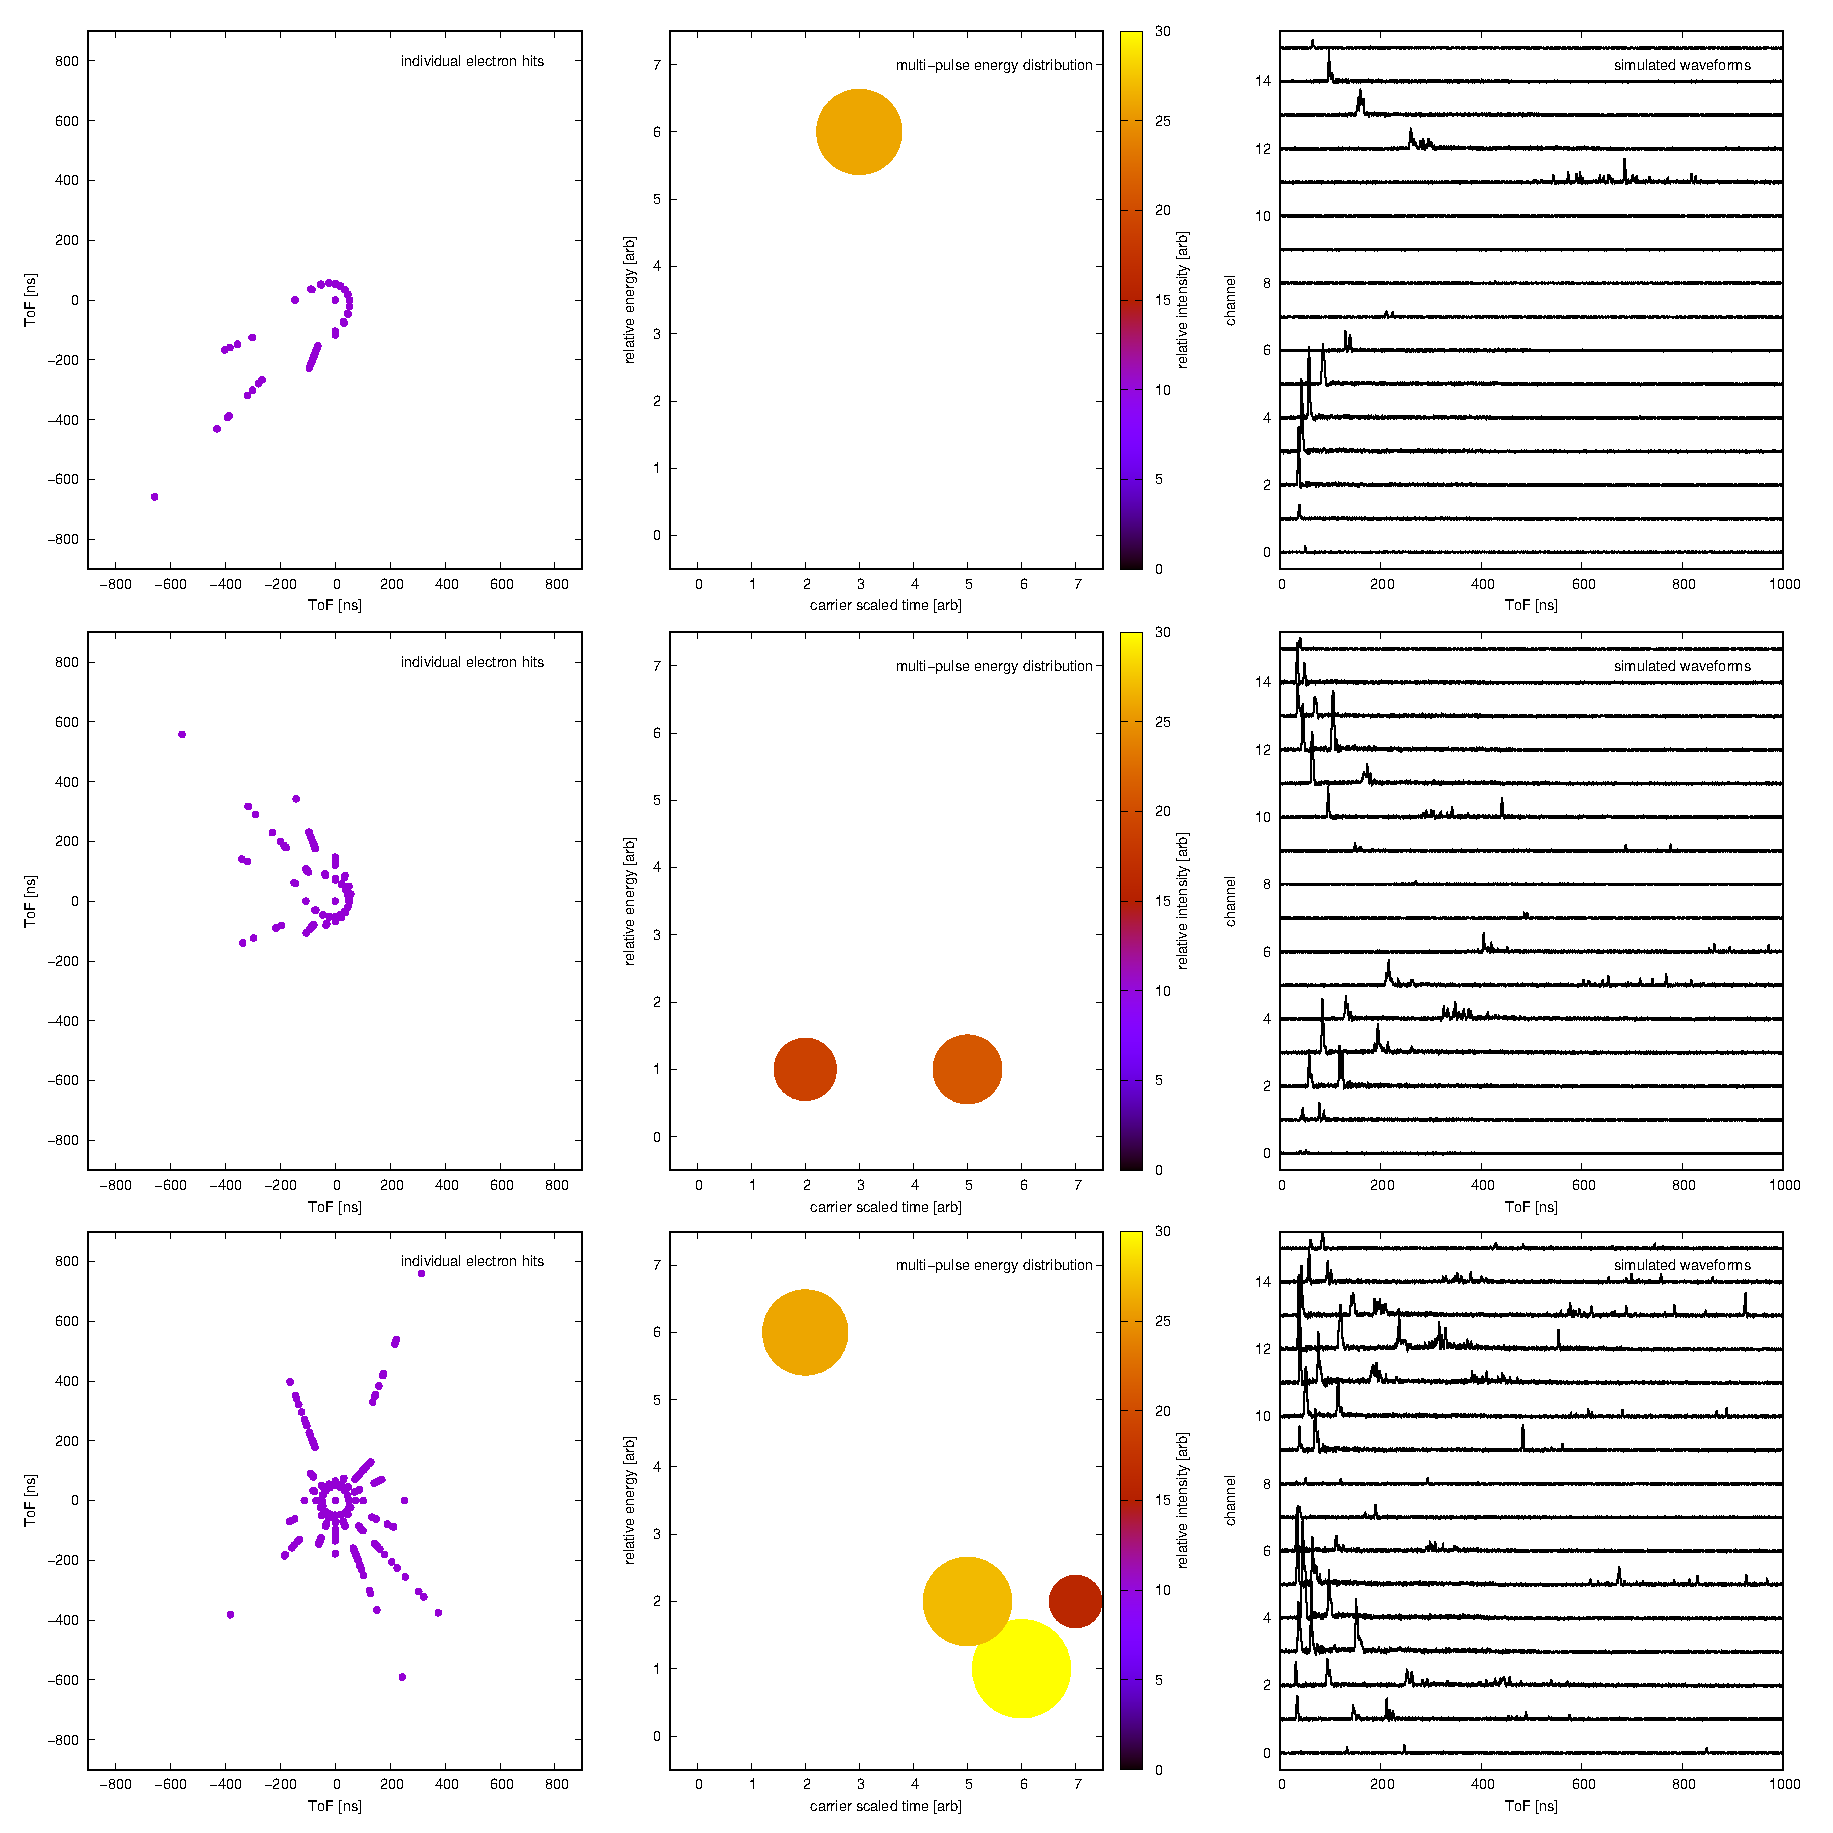
\includegraphics[trim={-2cm -2cm 0 0},width=\figwidth]{plotting.ToFs.eps}}
\caption{\label{fig::ToFs}
	(left) Electron arrival times in polar coordinates.
	(center) Multi-pulse time-energy (x-y) distributions of the x-ray pulses (point size and color indicate relative intensity).
	(right) Simulated ToF waveforms.
}
\end{figure}

In Ref.~\cite{Nick2018}, the previous generation of CookieBox was run in a 10s of electrons per shot counting regime in order that, given the much broader impulse response, the measured waveforms fairly closely represented the PDF for the outgoing photo-electrons.
A comparable hit-rate per shot was tested recently at the European XFEL, but for 1~MHz burst pulse rate which showed 10-fold signal degradation over the burst duration \cite{MarkusUpdate2019}.
Furthermore, we have chosen to increase the drift length in order to improve the spectral resolution over a broader energy window.
This increase in spectral resolution over a broader range of incoming electron energies has the draw back of poorer collection solid angle.
We also note that the high time-resolution Hamamatsu MCPs have a rather small 27~mm active area, thus even further restricting the collection angle.
We are therefore targeting a machine learning data analysis paradigm that is more amenable to under sampled PDFs.

\begin{figure}
\centerline{\includegraphics[trim={-3cm -2cm 1cm 1cm },clip,width=.8\figwidth]{plotting.debadri.eps}}
\caption{\label{fig::debadri}
Preliminary investigation into using Kernel Density Estimator.
% in order to quickly convert the under-sampled probability distribution function of photo-electrons to the desired input waveform for x-ray pulse shape inference.
}
\end{figure}

We are currently investigating Kernel Density Estimation (KDE) that could be implemented in the on-digitizer FPGA.
Ideally KDE would convert the sparsely sampled PDF for the outgoing photo-electrons into an estimated continuous form.
Represented in Fig.~\ref{fig::debadri}, one can easily see that in the ``pile-up'' regime where two distinct spectral features (red Gaussians) overlap, KDE results insufficiently represent the ``true'' PDF (red).
Our goal is to use machine learning to help jointly optimize the balance between x-ray pulse reconstruction accuracy and KDE bandwidth tuning in the pre-processing layer.

\section*{Edge Machine Learning}

Machine learning is a method of nonlinear curve fitting for very high dimensional data.
Well fitted models have been shown to be quite immune to (Gaussian) noise.
Although fitting the model, so-called ``training,'' is both data and simulation hungry and also computationally expensive and time-consuming, the application of the trained model involves a fairly straight forward sequence of matrix operations.
These matrix operations, the so-called ``inference,'' parallelize well under either GPU or FPGA instantiation. 
A portion of the raw data will be also transferred for use in model validation and subsequent re-training, and active models will be tightly bound to the data that they were used to produce.%, allowing for subsequent interrogation if there arises doubt regarding the quality of results.
Such near-detector FPGA-based inference engines we call Inference at the Edge or ``EdgeML.''

\begin{figure}
\centerline{\includegraphics[clip,width=.8\figwidth]{ConnectionDiagram_cookiebox_humaninloop_new.eps}}
\caption{\label{fig::humaninloop}
Current architecture for FPGA-based machine learning models.  
Early layers pre-analyze individual ToF channels independently and in parallel.
Deeper layers merge the results into the actionable information such as multi-pulse energy, delay, and polarization.
}
\end{figure}

Given the expected data rates for the LCLS-II(-HE) facilities, there is a growing EdgeML effort inside of LCLS that also has begun to extend to SSRL, High Energy Physics, and observational astronomy.  
Industry at large is entering an age where the velocity of data streams are becoming prohibitively high for expected network channels.
Given the potential for the CookieBox digitizers to produce a continuous data rate of over 200 GB/s, we are using the CookieBox project as a prescient use case for EdgeML.
This Edge Machine Learning project began with LDRD funding in FY18 and continues through FY19.

\begin{eqnarray}
\left[S_0, S_1 \cdots S_n\right] &\stackrel{\textrm{FPGA}}{\Longmapsfrom}& N_{\textrm{el}} (t) \stackrel{\textrm{Detector}}{\Longmapsfrom} \textrm{Event} \nonumber\\
\Downarrow\hspace{1cm}&&\hspace{1cm} \vec{\alpha} \stackrel{\textrm{Human}}{\Longmapsfrom} \textrm{Exp. Conditions}\nonumber\\
\Downarrow\hspace{1cm}&&\hspace{1cm} \Downarrow\nonumber\\
\left[S_0, S_1 \cdots S_n\right] &\stackrel{\textrm{Software}}{\Longmapsto}& \left[\tau_0 ,\tau_1 \cdots \tau_m \right] , \vec{\alpha} \nonumber\\%\stackrel{\textrm{Human}}{\Longmapsfrom} \textrm{Exp. Conditions}\\
   & &\hspace{1cm}\Downarrow \textrm{Software}\nonumber\\
 \textrm{Physical model} \stackrel{\textrm{Human}}{\Longmapsfrom} \expect{\mathcal{O} \left(\vec{\alpha}\right)} &\stackrel{\textrm{Simulation}}{\Longmapsfrom}& \mbox{Hist}\left( \mathcal{O} , \vec{\alpha} \right) \label{eqn::oldschool}
\end{eqnarray}

In the traditional case of data processing (Eq.~\ref{eqn::oldschool}), there are multiple levels where users leverage abstracted software to process incoming signals.
Detectors feed into digitized waveforms ($\left[S_0, S_1 \cdots S_n\right]$) by FPGA, with possible simple modifications.
The FPGAs then hand over digital waveforms to CPU based algorithms that convert signals into extracted parameters ($\left[\tau_0 ,\tau_1 \cdots \tau_m \right]$).
These parameters get combined with experimental conditions ($\vec{\alpha}$) for subsequent increment of a histogram ($\mbox{Hist}\left( \mathcal{O} , \vec{\alpha} \right)$) that the user hopes will represent some expectation value for an observable ($\expect{\mathcal{O} \left(\vec{\alpha}\right)}$).
We, on the other hand, take inspiration from Fig.~\ref{fig::hackernoon}.

There has been great recent progress with both in porting simple algorithms to Application Specific Integrated Circuits (ASICs) as well as compiling trained inference models to Field Programmable Gated Arrays (FPGAs) \cite{spatial}.  
When looking to industry, we see a clear trend to low-power, heavily parallelized, streaming data analysis \cite{hackernoon}.
This is driven by the coming evolution to so-called Industry 4.0, or the Industrial Internet of things (IIoT).
We plan to leverage SLAC's long history in ASIC and FPGA design to incorporate the machine learning analysis paradigm into the detector-side electronics.

\begin{figure}
\centerline{\includegraphics[clip,width=.8\linewidth]{hackernoon.ps}}
\caption{\label{fig::hackernoon}
Cartoon from \cite{hackernoon} representing the growing importance of Edge compute solutions like FPGAs and ASICs for processing intensive tasks (blockchain in this case).
}
\end{figure}

We expect that with sufficient model training one could move directly from raw signal to an updated representation of the physical observable $\expect{\mathcal{O} \left(\vec{\alpha}\right)}$ (Eq.~\ref{eqn::newschool})
Of course, such an analysis chain would require adaptability and thus will likely not fit completely into the on-detector FPGA.
We adopt a co-design approach, leveraging the particular strengths of each piece of computational hardware, e.g. ASICs an FPGAs on the sensor along with FPGAs and GPUs further along the data stream.

 \begin{eqnarray}
 &\textrm{Exp. Conditions}&\nonumber \\
   & \hspace{1cm}\Downarrow & \label{eqn::newschool}\\%\textrm{Detectors}\\
 \textrm{Physical model} \stackrel{\textrm{Human}}{\Longmapsfrom} \expect{\mathcal{O} \left(\vec{\alpha}\right)} \stackrel{\textrm{FPGA}}{\Longmapsfrom} & \left[N_{\textrm{el}} (t)  , \vec{\alpha}\right] & \Longmapsfrom \textrm{Event} \nonumber
 \end{eqnarray}

Users, domain experts for their own experiments, are the target audience for our development environment, one that exposes examples of detector inference and training.
We expect proficient users will build their own inference models that can be compiled and deployed to our FPGAs in preparation for their beamtimes.
As depicted in Fig.~\ref{fig::highlevel}, we are standardizing on Docker as a computing environment image. %that can be shared with user institutions.
These images enable the user to develop at home inside a containerized computing environment that is identical to what he of she will encounter here at LCLS.
Users will also have access to FPGA resources and the high-level compiler stack known as Spatial \cite{spatial} in order to facilitate early benchmarking of algorithms on the same FPGA hardware as will be featured in the LCLS-II data stream.

\begin{figure}
\centerline{\includegraphics[clip,width=.8\linewidth]{HighLevel_new.eps}}
\caption{\label{fig::highlevel}
Exposing the FPGA development environment to the broader user community as well as enabling Leadership Computing facilities for accelerate the ML Training.
}
\end{figure}

\bibliographystyle{unsrt}
\bibliography{$BIBFILES/Coffee,$BIBFILES/computing}

\section*{Acknowledgements}
%It is under B&R (Budget & Reporting) code KC0406020.
This work is supported by the U.S. Department of Energy, Office of Science, Office of Basic Energy Sciences under Contract No. DE-AC02-76SF00515.
The CookieBox effort is supported under the Accelerator and Detector Research program of the U.S. Department of Energy, Office of Science.
The EdgeML effort is supported by the Department of Energy, Laboratory Directed Research and Development program at SLAC National Accelerator Laboratory.
Feldman is supported by the Stanford Graduate Fellowship in Science and Engineering.
Corbeil-Therrien is partially supported through a Banting Postdoctoral Fellowship from the Government of Canada.


\end{document}
